\documentclass[border=0, var width]{standalone}
\usepackage{tikz}
\usetikzlibrary{arrows,calc,matrix,scopes}
% define simple color names for esa colors and a highlight
\definecolor{esa}{RGB}{10,156,215}
\def\esacolorfactor{20}
\colorlet{esa0}{esa!90!white}
\colorlet{esa1}{black!\esacolorfactor!esa0}
\colorlet{esa2}{black!\esacolorfactor!esa1}
\colorlet{esa3}{black!\esacolorfactor!esa2}
\colorlet{esa4}{black!\esacolorfactor!esa3}
\colorlet{esa5}{black!\esacolorfactor!esa4}
\definecolor{highlight}{RGB}{189,27,27}


\renewcommand\rmdefault{\sfdefault}

\begin{document}
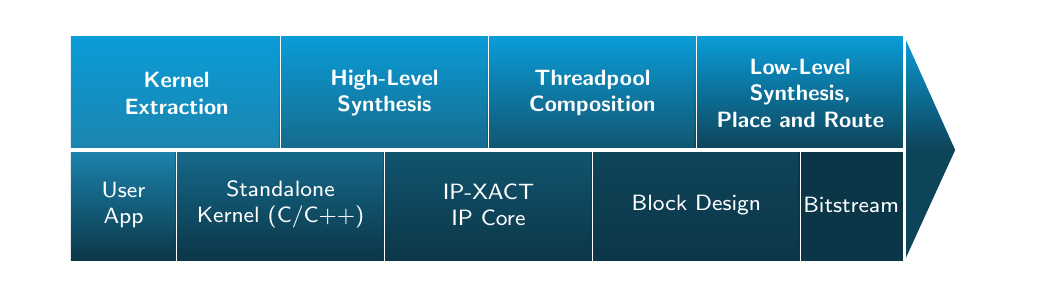
\begin{tikzpicture} [ %
  us/.style={shade, bottom color=esa1, top color=esa}, %
  ls/.style={shade, top color=esa1, bottom color=esa5}] %
\matrix (m2) [matrix of nodes, ampersand replacement=\&, column sep=-\pgflinewidth, %
  row sep=-\pgflinewidth, nodes={rectangle, text width=1.1cm, align=center}, %
  text depth=1.25ex, text height=1cm, nodes in empty cells] { %
  |[us]| \& |[us]| \& %
  |[us, bottom color=esa2]| \& |[us, bottom color=esa2]| \&  %
  |[us, bottom color=esa3]| \& |[us, bottom color=esa3]| \& %
  |[us, bottom color=esa4]| \& |[us, bottom color=esa4]| \&\\ %
  |[ls]| \&  %
  |[ls, top color=esa2]| \& |[ls, top color=esa2]| \&  %
  |[ls, top color=esa3]| \& |[ls, top color=esa3]| \& %
  |[ls, top color=esa4]| \& |[ls, top color=esa4]| \& %
  |[ls, top color=esa5]| \&\\ %
}; %
\shade [top color=esa, bottom color=esa4, middle color=esa4] %
  (m2-1-8.north east) -- (m2-2-8.south east) -- (m2-1-9.south) -- cycle; %
\draw [-, very thick, white] (m2-1-1.south west) -- (m2-1-8.south east); %
\draw [-, very thick, white] (m2-1-8.north east) -- (m2-2-8.south east); %
\foreach \col in {2,4,6,8} \draw[-, thin, white] (m2-1-\col.north east) -- (m2-1-\col.south east); %
\foreach \col in {1,3,5,7} \draw[-, thin, white] (m2-2-\col.north east) -- (m2-2-\col.south east); %
 %
\begin{scope}[every node/.style={font=\footnotesize\color{white}, align=center, text width=2.2cm}] %
  \node at (m2-2-1) {User\\App}; %
  \node at (m2-1-1.east) {\bf Kernel\\Extraction}; %
  \node at (m2-2-2.east) {Standalone\\Kernel (C/C++)}; %
  \node at (m2-1-3.east) {\bf High-Level\\Synthesis}; %
  \node at (m2-2-4.east) {IP-XACT\\IP Core}; %
  \node at (m2-1-5.east) {\bf Threadpool\\Composition}; %
  \node at (m2-2-6.east) {Block Design}; %
  \node [text width=2.4cm] at (m2-1-7.east) {\bf Low-Level\\Synthesis,\\Place and Route}; %
  \node at (m2-2-8) {Bitstream}; %
\end{scope} %
\end{tikzpicture} %
\end{document}
